
\begin{minipage}{0.68\linewidth}
Le jeu de Franc-carreau

Pour jouer au jeu de franc-carreau, on dispose d’un damier constitué de carreaux de forme carrée de 5 cm de côté et d’une pièce de 50 millimes de dinars, dont le rayon est 1,2 cm. Le jeu consiste à lancer la pièce au hasard sur le damier. 
Si la pièce ne chevauche pas les lignes du quadrillage, on dit alors que la pièce est à franc-carreau. 
Si le centre de la pièce est à l’extérieur du damier, alors le lancer ne compte pas et on recommence le lancer.
\end{minipage}
\hfill
\begin{minipage}{0.28\linewidth}
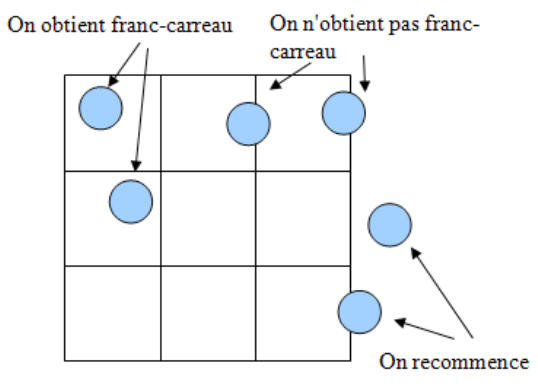
\includegraphics[scale=0.3]{Franc-carreaux.png} 
\end{minipage}

\begin{enumerate}
\item  Effectuer une série de 10 lancers et noter pour chaque lancer 1 si on obtient franc-carreau et 0 sinon.  \point{1}
\item  Calculer la fréquence de francs-carreaux obtenue. Comparer les fréquences obtenues par les autres élèves de la classe. \point{1}

\item Sur tableur, réaliser le tableau suivant puis compléter les deux premières lignes où l’on cumule, élève après élève, le nombre de lancers et le nombre de francs-carreaux.


Regrouper par binôme les résultats et recopier le tableau ici :

\begin{tabular}{|c|p{4.5cm}|*{15}{c|}}
\hline 
 & A & B & C & D & E & F & G & H & I & J & K & L & M & N & O  & P   \\ 
\hline 
1&  Elève & 1 & 2 & 3 & 4 & 5 & 6 & 7 & 8 & 9 & 10 & 11 & 12 & 13 & 14 & 15    \\ 
\hline 
2&Lancer & 20 & 40 & 60 & 80 &  &  & &  &  &  &  &  &  &  &     \\ 
\hline 
3&Nbre de Franc-carreaux &  &  &  &  &  &  & &  &  &  &  &  &  &  &   \\ 
\hline 
4&Freq cumulées croissantes &  &  &  &  &  &  & &  &  &  &  &  &  &  &     \\ 
\hline 
\end{tabular} 

\item  
\begin{enumerate}
\item  Quelle formule peut-on écrire dans la cellule C2 pour compléter la ligne 2 en la recopiant vers la droite ? \point{1}
\item  Quelle formule peut-on insérer dans la cellule B4 afin de pouvoir remplir la ligne 4 en la recopiant vers la droite ? \point{1}
\item  


\begin{minipage}{0.18\linewidth}
Construire le graphique représentant la fréquence de franc-carreaux obtenus en fonction du nombre de lancers pris en compte sur le repère ci-contre.
\item  Quelle semble être la probabilité de franc-carreau ? 
\end{minipage}
\hfill
\begin{minipage}{0.78\linewidth}

\definecolor{cqcqcq}{rgb}{0.7529411764705882,0.7529411764705882,0.7529411764705882}
\begin{tikzpicture}[line cap=round,line join=round,>=triangle 45,x=0.030963136043150423cm,y=7.187955203828905cm]
\draw [color=cqcqcq,, xstep=0.6192627208630085cm,ystep=1.4375910407657813cm] (-14.51458566395133,-0.061378216267091563) grid (308.4501161693493,1.0515947744018725);
\draw[->,color=black] (-14.51458566395133,0.) -- (308.4501161693493,0.);
\foreach \x in {,20.,40.,60.,80.,100.,120.,140.,160.,180.,200.,220.,240.,260.,280.,300.}
\draw[shift={(\x,0)},color=black] (0pt,2pt) -- (0pt,-2pt) node[below] {\footnotesize $\x$};
\draw[->,color=black] (0.,-0.061378216267091563) -- (0.,1.0515947744018725);
\foreach \y in {,0.2,0.4,0.6,0.8,1.}
\draw[shift={(0,\y)},color=black] (2pt,0pt) -- (-2pt,0pt) node[left] {\footnotesize $\y$};
\draw[color=black] (0pt,-10pt) node[right] {\footnotesize $0$};
\clip(-14.51458566395133,-0.061378216267091563) rectangle (308.4501161693493,1.0515947744018725);
\end{tikzpicture}

\end{minipage}



\end{enumerate}
\item ABCD représente un carré de 5 cm du damier.
\begin{enumerate}

\item  Dessiner ce carré. Colorier ensuite la zone pour laquelle le franc-carreau n’est pas réalisé. 
\item  Calculer alors la probabilité de franc-carreau puis la comparer avec le graphique de la question précédente.
\end{enumerate}

\end{enumerate}

\newpage

\definecolor{xdxdff}{rgb}{0.49019607843137253,0.49019607843137253,1.}
\begin{tikzpicture}[line cap=round,line join=round,>=triangle 45,x=1.0cm,y=1.0cm]
\draw [line width=1.pt] (0,-10) -- (0,15);
\draw [line width=1.pt] (5,-10) -- (5.,15);
\draw [line width=1.pt] (10,-10) -- (10.,15);
\draw [line width=1.pt] (15,-10) -- (15.,15);

\draw [line width=1.pt] (0,15) -- (15,15);
\draw [line width=1.pt] (0,10) -- (15.,10);
\draw [line width=1.pt] (0,5) -- (15.,5);
\draw [line width=1.pt] (0,0) -- (15.,0);
\draw [line width=1.pt] (0,-5) -- (15.,-5);
\draw [line width=1.pt] (0,-10) -- (15.,-10);
\begin{scriptsize}
\end{scriptsize}
\end{tikzpicture}